%%%%%%%%%%%%%%%%%%%%%%%%%%%%%%%%%%%%%%%%%
% Election Computing System
% System obliczający i wizualizujący wyniki zgodnie z uogólnieniem systemu k-Borda na podstawie norm ell_p.
%
% Prezentacja wykonana na Pracownię Projektową
%
%%%%%%%%%%%%%%%%%%%%%%%%%%%%%%%%%%%%%%%%%

%----------------------------------------------------------------------------------------
%	PACKAGES AND THEMES
%----------------------------------------------------------------------------------------

\documentclass{beamer}

\usepackage[T1]{fontenc}
\usepackage[polish]{babel}
\usepackage[utf8]{inputenc}
\usepackage{lmodern}
\usepackage{amsmath}
\usepackage{algorithm2e}

\selectlanguage{polish}

\mode<presentation> {
	\usetheme{Copenhagen}
}

\usepackage{graphicx} % Allows including images
\usepackage{booktabs} % Allows the use of \toprule, \midrule and \bottomrule in tables


% Custom macros

\newcommand{\red}[1]{
	{ \color{red}{#1} }
}

\newcommand{\score}[2]{
	\stackrel
	{\red{#1}}
	{#2}
}

\definecolor{links}{HTML}{2A1B81}
\hypersetup{colorlinks,linkcolor=,urlcolor=links}


%----------------------------------------------------------------------------------------
%	TITLE PAGE
%----------------------------------------------------------------------------------------

\title
[System obliczający wyniki wyborów]
{System obliczający wyniki wyborów dla uogólnienia systemu k-Borda}

\author
[T. Kasprzyk, D. Ogiela, J. Stępak]
{Tomasz Kasprzyk, \ Daniel Ogiela, \ Jakub Stępak}

\institute
[AGH]
{
Akademia Górniczo-Hutnicza

Wydział Informatyki, Elektroniki i Telekomunikacji

Katedra Informatyki 
\newline \newline
Projekt realizowany pod opieką \\dr. hab. inż. Piotra Faliszewskiego

}
\date{26 stycznia 2017}

%----------------------------------------------------------------------------------------

\begin{document}

\frame{\titlepage}

%\begin{frame}
%\frametitle{Plan}
%\tableofcontents
%\end{frame}

%----------------------------------------------------------------------------------------
%	PRESENTATION SLIDES
%----------------------------------------------------------------------------------------

%------------------------------------------------
\section{Opis problemu}
%------------------------------------------------

\subsection{Definicja wyborów}

%------------------------------------------------

\begin{frame}
\frametitle{Definicja wyborów}
Wybory to para $E = (C, V)$,
gdzie $C = \{ c_1, c_2, \ldots, c_m \}$ to zbiór kandydatów,
a $V = (v_1, v_2, \ldots, v_n)$ to ciąg wyborców.
Każdy wyborca posiada swoje $preferencje$,
które są ciągiem kandydatów w porządku od najbardziej preferowanego
przez danego wyborcę do najmniej preferowanego. Ponadto dana jest liczba $k$, będąca wielkością wybieranego komitetu.
\end{frame}

%------------------------------------------------

\subsection{Przykładowe wybory}
\begin{frame}
\frametitle{Przykładowe wybory}
\begin{exampleblock}{Wybory filmów}


$ C = \{$komedia, horror, film akcji, dramat, science fiction$\} $ \\
$ V = ($Anna, Jan, Piotr, Paweł$) $ \\ ~ \\
 \textbf{Anna:}  $\score{1}{dramat} \ > \ \score{2}{komedia} \ > \ \score{3}{film \ akcji} \ > \ \score{4}{horror} \ > \ \score{5}{science \ fiction}$\\
 \textbf{Jan:}  $\score{1}{science \ fiction} \ > \ \score{2}{komedia} \ > \ \score{3}{dramat} \ > \ \score{4}{film \ akcji} \ > \ \score{5}{horror}$ \\
 \textbf{Piotr:} $\score{1}{horror} \ > \ \score{2}{dramat} \ > \ \score{3}{film \ akcji} \ > \ \score{4}{komedia} \ > \ \score{5}{science \ fiction}$\\
 \textbf{Paweł:} $\score{1}{science \ fiction} \ > \ \score{2}{film \ akcji} \ > \ \score{3}{komedia} \ > \ \score{4}{horror} \ > \ \score{5}{dramat}$\\ ~ \\
$ k = 2 $


\end{exampleblock}
\end{frame}

%------------------------------------------------
\subsection{Pojęcia pomocnicze}

\begin{frame}
\frametitle{Punktacja Bordy}

Niech $v$ będzie głosem nad zbiorem kandydatów $C$.
Punkty przyporządkowane każdemu kandydatowi $c \in C$ w $v$ wynoszą
$||C|| - pos_v(c)$, gdzie $pos_v(c)$ to pozycja kandydata $c$ w $v$.

\begin{exampleblock}{Funkcja Bordy}
$$
\beta(i) = m-i, \quad gdzie \ m = ||C||
$$
\end{exampleblock}

\begin{exampleblock}{Preferencje wyborcy}
$$ 
v_1: \score{m-1}{c_1} \ > \ \score{m-2}{c_2} \ > \ \score{m-3}{c_3} \ > \ \score{m-4}{c_4} \ > \ \ldots
$$
\end{exampleblock}

\end{frame}

%------------------------------------------------

\begin{frame}
\frametitle{Ciąg pozycji}

Dla wybranego komitetu $S$ i danego
wyborcy $v$ definiujemy ciąg $pos_v(S) $ jako
posortowany ciąg pozycji, które zajmują kandydaci z $S$ w preferencjach wyborcy $v$. \\ 
\vspace{\baselineskip}
Niech $S = \{c_1, c_3, c_5, c_6\}$

\begin{exampleblock}{Preferencje wyborcy}
$$
v_1: \ \score{1}{c_5} \ > \ \score{2}{c_3} \ > \ \score{3}{c_1} \ > \ \score{4}{c_2} \ > \ \score{5}{c_6} \ > \ \score{6}{c_4} > \ldots
$$
\end{exampleblock}

$$pos_{v_1}(S) = (1, 2, 3, 5)$$

\begin{exampleblock}{Oznaczenie wartości funkcji satysfakcji}
$$
f(i_1, \ldots, i_k)
$$
\end{exampleblock}

\end{frame}

%------------------------------------------------

%\begin{frame}
%\frametitle{Committee scoring rules}

%Istnieją systemy wyborcze: \\ ~ \\

%\begin{tabular}{ll}
%k-Borda: 			& $f_{kB}(i_1, \ldots, i_k) = \beta(i_1) + \ldots + \beta(i_k)$\\
%Chamberlin–Courant:  & $f_{CC}(i_1, \ldots, i_k) = \beta(i_1)$
%\end{tabular}

%\end{frame}

%------------------------------------------------

\begin{frame}
\frametitle{Norma $\ell_p$}
Niech $x_1, x_2, \ldots , x_n \in \mathbb{R}, p \in \mathbb{N}$
\begin{block}{Norma $\ell_p$}
$$
\ell_p(x_1, x_2, \ldots, x_n ) = \sqrt[p]{ x_1^p + x_2^p + \ldots + x_n^p }
$$
\end{block}

\begin{exampleblock}{}
$$
\begin{aligned}
\ell_1 	\	 &\equiv 	\ \ +  \\
\ell_\infty 	\  &\equiv 	\ max 
\end{aligned}
$$
\end{exampleblock}

\end{frame}

%------------------------------------------------

\subsection{System $\ell_p-Borda$}
\begin{frame}
\frametitle{System $\ell_p-Borda$}

\begin{block}{Funkcja satysfakcji $\ell_p-Borda$}
$$
f_{\ell_p}(i_1, i_2, \ldots, i_k ) = \ell_p(\beta(i_1), \beta(i_2), \ldots ,\beta(i_k))
$$
\end{block}
\vspace{\baselineskip}
\vspace{\baselineskip}

\begin{exampleblock}{Funkcja satysfakcji k-Borda (gdy $p = 1$)}
$$
f_{k-Borda}(i_1, \ldots, i_k) = \beta(i_1) + \ldots + \beta(i_k)
$$
\end{exampleblock}

\begin{exampleblock}{Funkcja satysfakcji Chamberlina-Couranta (gdy $p \to \infty$)}
$$
f_{CC}(i_1, \ldots, i_k) = \beta(i_1)
$$
\end{exampleblock}

%\begin{exampleblock}{}
%$$
%\begin{aligned}
%f_{\ell_1} 	\	 &\equiv 	f_{k-Borda}  \\
%f_{\ell_\infty} 	\  &\equiv 	\ f_{Chamberlin-Courant} 
%\end{aligned}
%$$
%\end{exampleblock}

\end{frame}

\section{Opis systemu}
\subsection{Konto użytkownika}
\begin{frame}
\frametitle{Konto użytkownika}

\includegraphics[width=0.9\paperwidth]{pics/home_page.png}
\end{frame}

\subsection{Wprowadzanie danych o wyborach}
\begin{frame}
\frametitle{Metody wprowadzania danych}
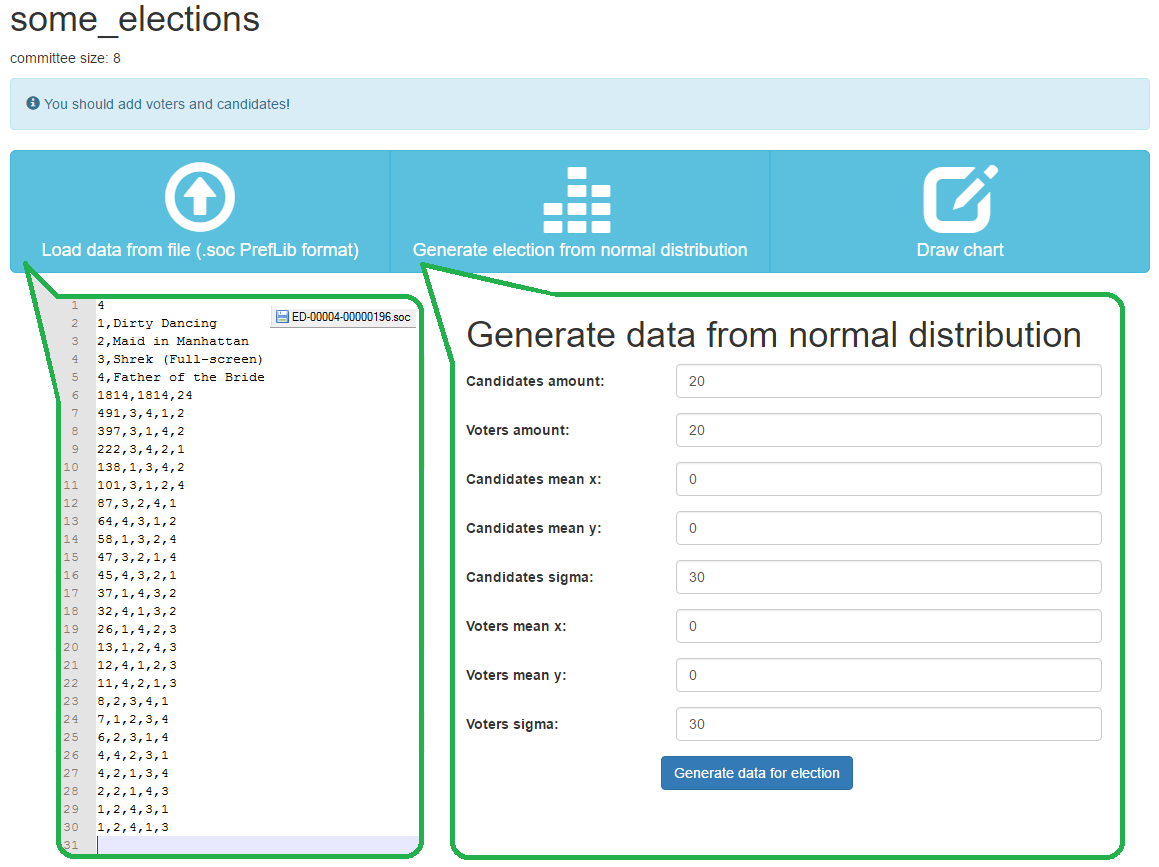
\includegraphics[width=0.7\paperwidth]{pics/three_options.png}
\end{frame}

\begin{frame}
\frametitle{Zaznaczanie punktów na płaszczyźnie}
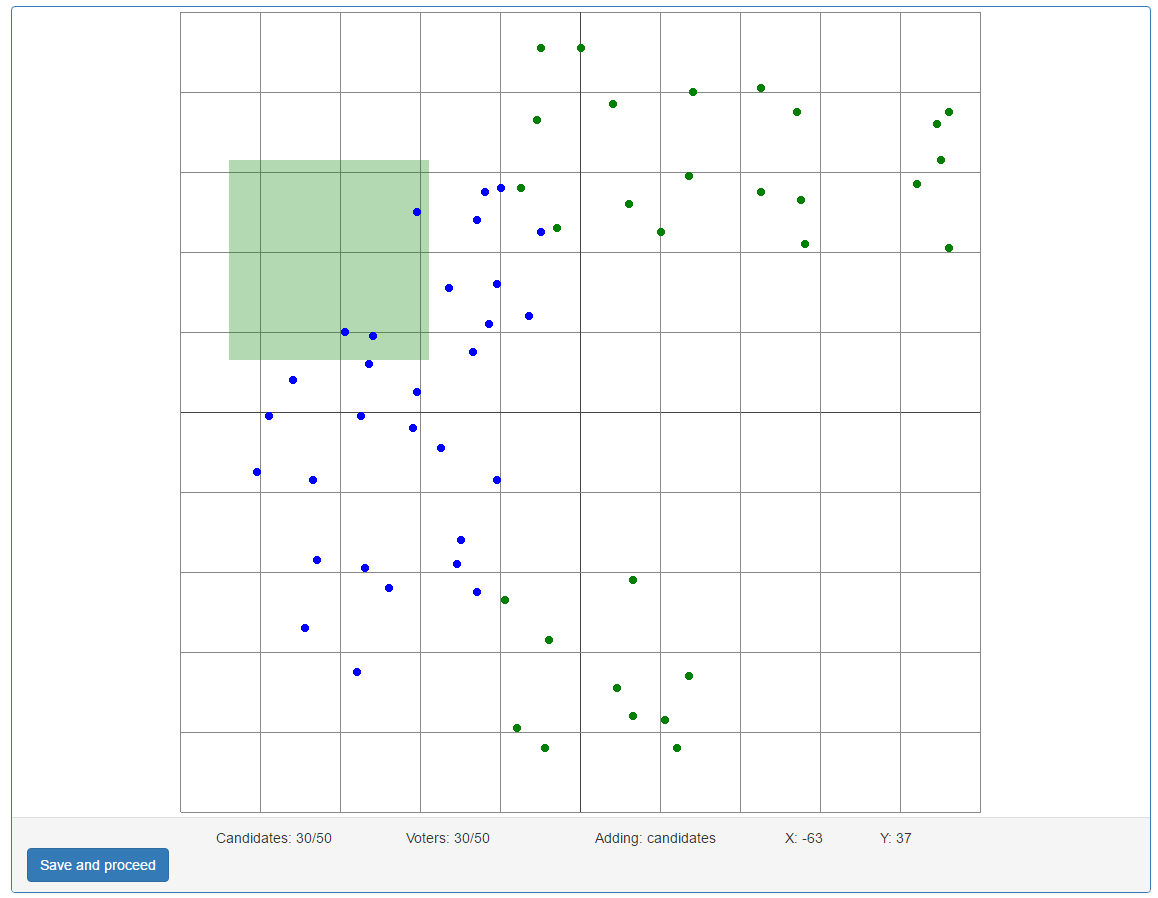
\includegraphics[width=0.7\paperwidth]{pics/paint.png}
\end{frame}

\subsection{Obliczanie wyników}
\begin{frame}
\frametitle{Dobór parametrów do obliczeń}
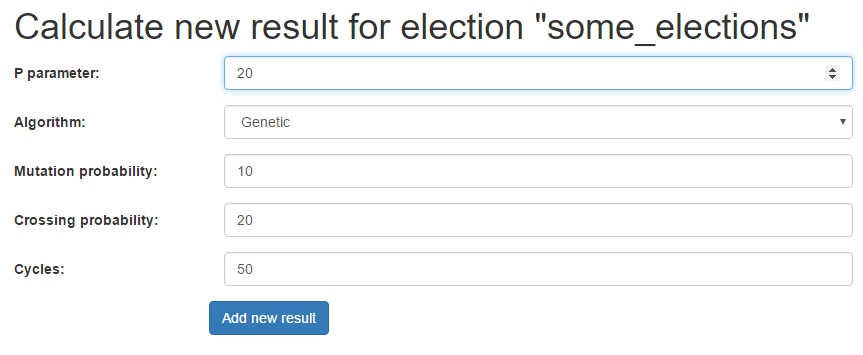
\includegraphics[width=0.9\paperwidth]{pics/parameters.png}
\end{frame}

\subsection{Prezentacja wyników}
\begin{frame}
\frametitle{Rozmieszczenie kandydatów, wyborców i zwycięzców}
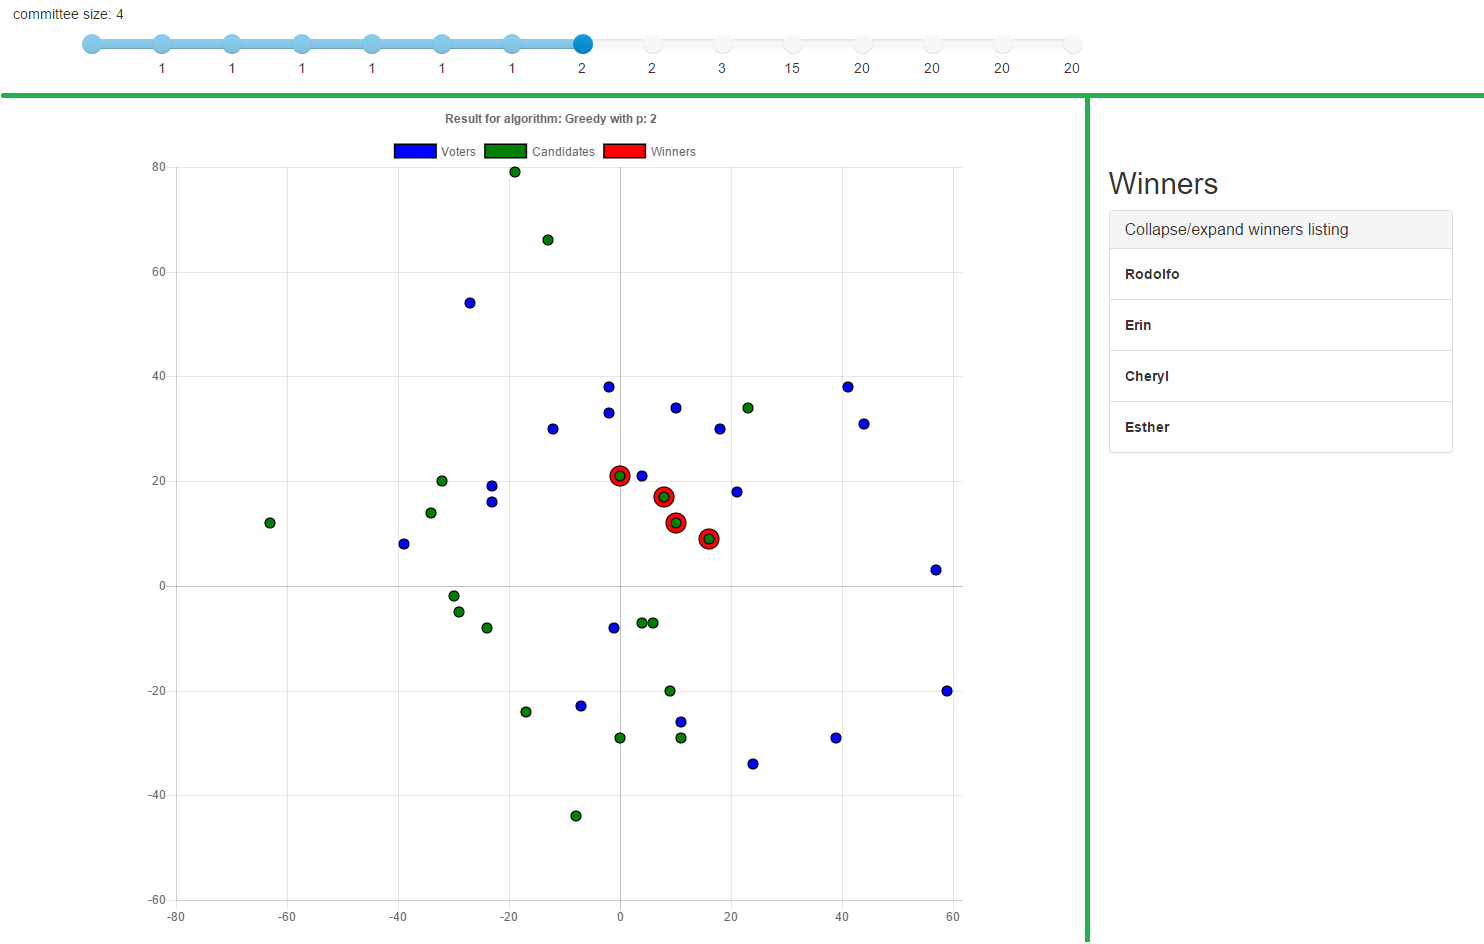
\includegraphics[width=0.80\paperwidth]{pics/chart_with_slider_and_winners.png}
\end{frame}

\begin{frame}
\frametitle{Rozmieszczenie kandydatów, wyborców i zwycięzców}
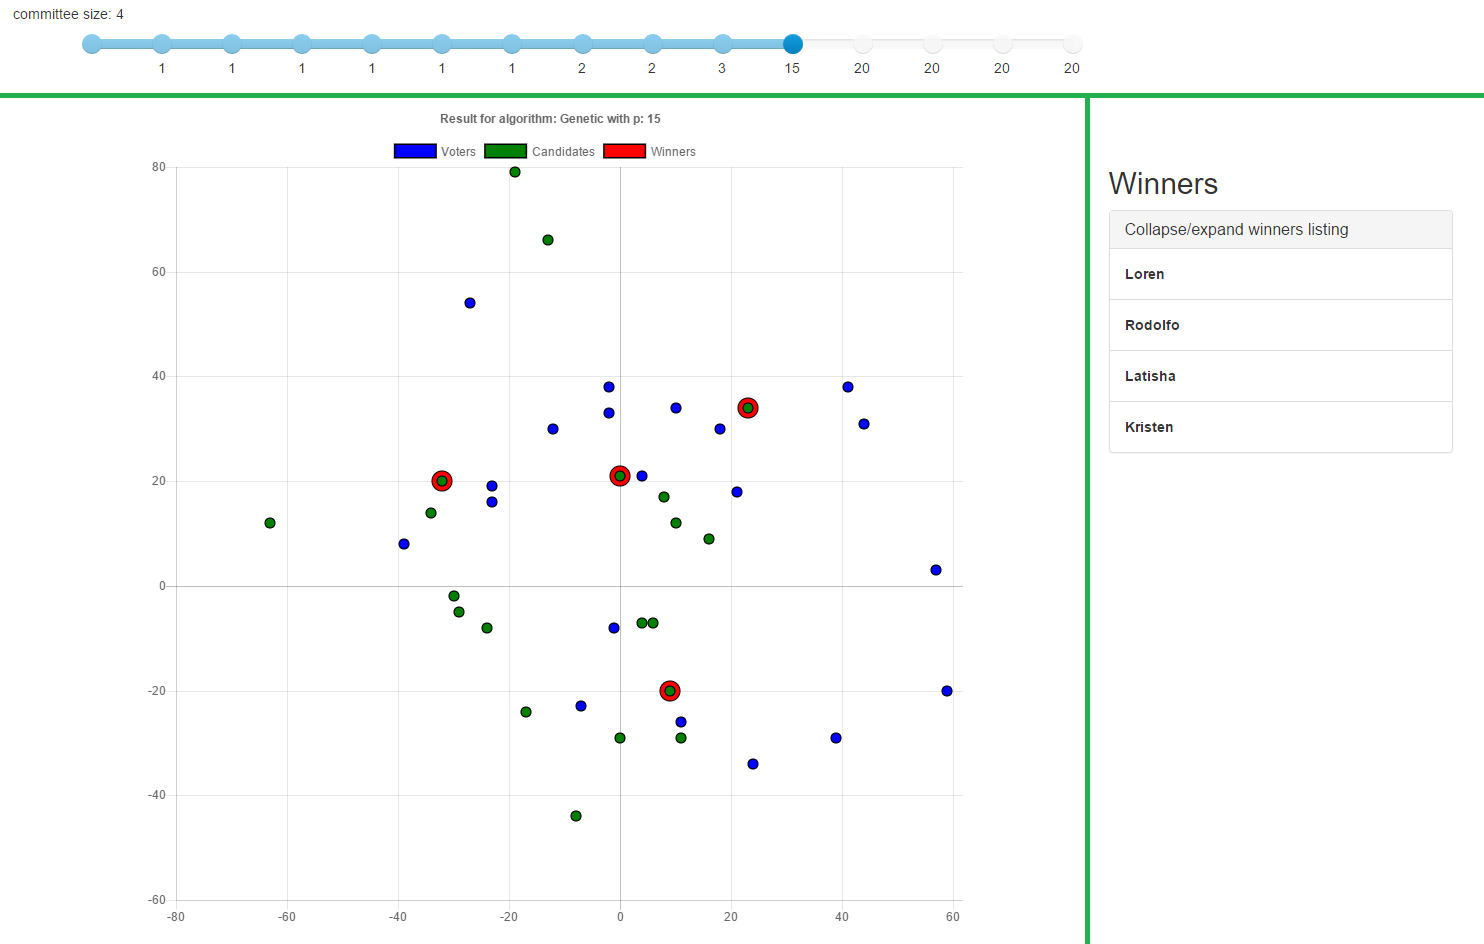
\includegraphics[width=0.80\paperwidth]{pics/chart_with_slider_and_winners_2.png}
\end{frame}

\begin{frame}
\frametitle{Porównanie wyników dla różnych algorytmów}
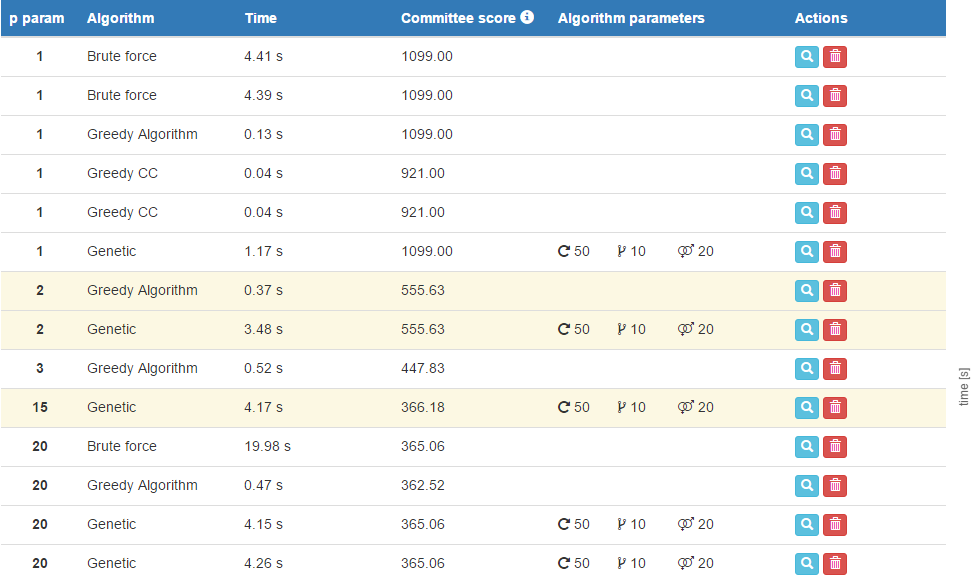
\includegraphics[width=0.85\paperwidth]{pics/algorithms_comparison_table.png}
\end{frame}

\begin{frame}
\frametitle{Porównanie wyników dla różnych algorytmów}
\begin{center}
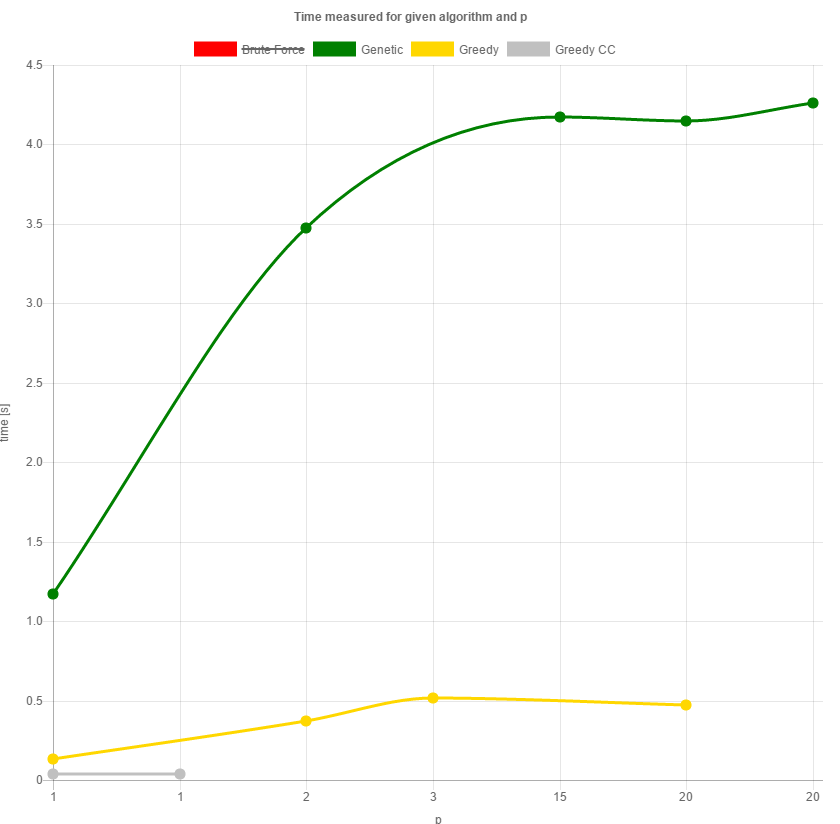
\includegraphics[width=0.5\paperwidth]{pics/p_t_chart.png}
\end{center}
\end{frame}


\section{Opis algorytmów}
\subsection{Algorytm brute-force}
\begin{frame}
\frametitle{Algorytmm brute-force}
\begin{algorithm}[H]
\SetAlgoLined
\KwData{$K$ - zbiór wszystkich możliwych komitetów w danych wyborach}
\KwResult{$REZULTAT$ - zwycięski zbiór $k$ kandydatów}
~\\
$REZULTAT \longleftarrow \emptyset $ \\
$najlepszy\_wynik \longleftarrow $ 0 \\
\For{$k \in K$ }{ ~\\
	\If{$wynik(k) > najlepszy\_wynik$}{ ~\\
		$REZUTLAT \longleftarrow k$ \\
		$najlepszy\_wynik \longleftarrow wynik(k)$
	}
}
\Return{$REZULTAT$}
\end{algorithm}
\end{frame}

\subsection{Algorytmy zachłanne}
\begin{frame}
\frametitle{Algorytm zachłanny zależny od parametru $p$}

\begin{algorithm}[H]
%\SetAlgoLined
\For{$i \longleftarrow 1$ to $k$ }{
	\For{$c \in C\setminus REZULTAT$}{
		\For{$v \in V$}{
		$dodaj\_zadowolenie\_wyborcy(v, REZULTAT \cup c)$\;
		}
		\If{$badany\_kandydat\_najlepszy(c)$}{
		$uaktualnij\_lidera\_iteracji(c)$\;
		}
	}
	$REZULTAT \longleftarrow REZULTAT \cup zwyciezca\_iteracji$\;
}
\Return{$REZULTAT$}
\end{algorithm}

\end{frame}

\begin{frame}
\frametitle{Algorytm zachłanny wg zasady $Chamberlina-Couranta$}
\begin{itemize}
\item niezależny od parametru $p$
\item aproksymacja wg funkcji satysfakcji $Chamberlina-Couranta$
\item schemat działania identyczny jak wcześniejszego algorytmu
\item zdecydowanie szybszy od głównego algorytmu zachłannego
\item dobra aproksymacja systemu $\ell_p-Borda$ dla dużych wartości parametru $p$   
\end{itemize}

\end{frame}

%----------------------------------------------------------------------------------------

\subsection{Algorytm genetyczny}

\begin{frame}
\frametitle{Osobnik}
Jako początkową populację osobników przyjmujemy 50 losowo wybranych komitetów.

~ \\ ~ \\ ~ \\


\includegraphics[width=0.8\paperwidth]{pics/committee.png}


\end{frame}


%----------------------------------------------------------------------------------------

\begin{frame}
\frametitle{Krzyżowanie i mutacja}
Podczas krzyżowania dwa osobniki wymieniają się losowo kandydatami. Tworzony jest nowy osobnik, zawierający k kandydatów którzy poprzednio byli w co najmniej jednym z osobników przystępujących do krzyżowania.

~ \\ 


\includegraphics[width=0.8\paperwidth]{pics/crossing.png}

Podczas mutacji jeden z kandydatów w osobniku jest wymieniany na innego, niebędącego dotąd w danym osobniku.

~ \\


\includegraphics[width=0.8\paperwidth]{pics/mutation.png}

\end{frame}

%----------------------------------------------------------------------------------------

\begin{frame}
\frametitle{Cykl}

Na jeden cykl algorytmu składa się:

\begin{itemize}
\item wybór par osobników do krzyżowania się
\item krzyżowanie osobników
\item mutacja osobników zgodnie z zadanym prawdopodobieństwem
\item wybór N osobników do przejścia do kolejnego cyklu
\end{itemize}

Liczba N określa wielkość puli osobników i jest wybierana na początku działania algorytmu. W naszej implementacji przyjęto stałą liczbę $50$ osobników.

\end{frame}

%----------------------------------------------------------------------------------------

\begin{frame}
\frametitle{Parametry algorytmu}

System pozwala wybrać:
\begin{itemize}
\item liczbę cykli działania algorytmu
\item część puli jaka jest poddawana krzyżowaniu (osobniki są z niej losowo wybierane do krzyżowania)
\item prawdopodobieństwo wystąpienia mutacji w pojedynczym osobniku
\end{itemize}
\end{frame}

%----------------------------------------------------------------------------------------

\section{Porównanie algorytmów}

\subsection{Charakterystyka algorytmów zachłannych}

\begin{frame}
\frametitle{Algorytmy zachłanne}

Jak duży musi być parametr $p$, by algorytm zachłanny wg zasady $Chamberlina - Couranta$ dawał dobre wyniki?

\begin{itemize}
\item Nie można definitywnie wyznaczyć granicy,
\item Dla $p = 50$ około 90\% wyników pokrywało się.
\end{itemize}

\end{frame}

%----------------------------------------------------------------------------------------

\subsection{Charakterystyka algorytmu genetycznego}

\begin{frame}
\frametitle{Algorytm genetyczny}

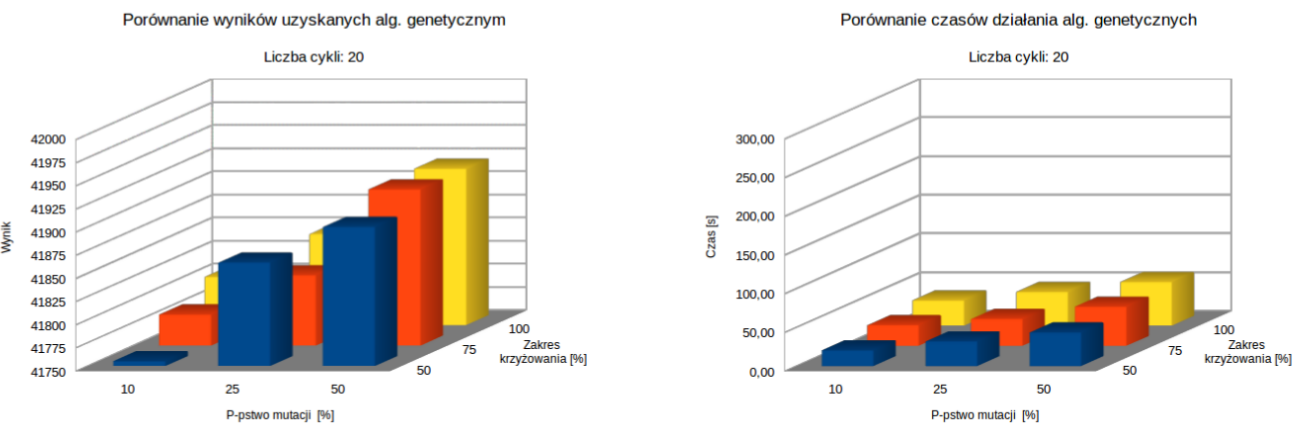
\includegraphics[width=0.8\paperwidth]{pics/gen20.png} \\

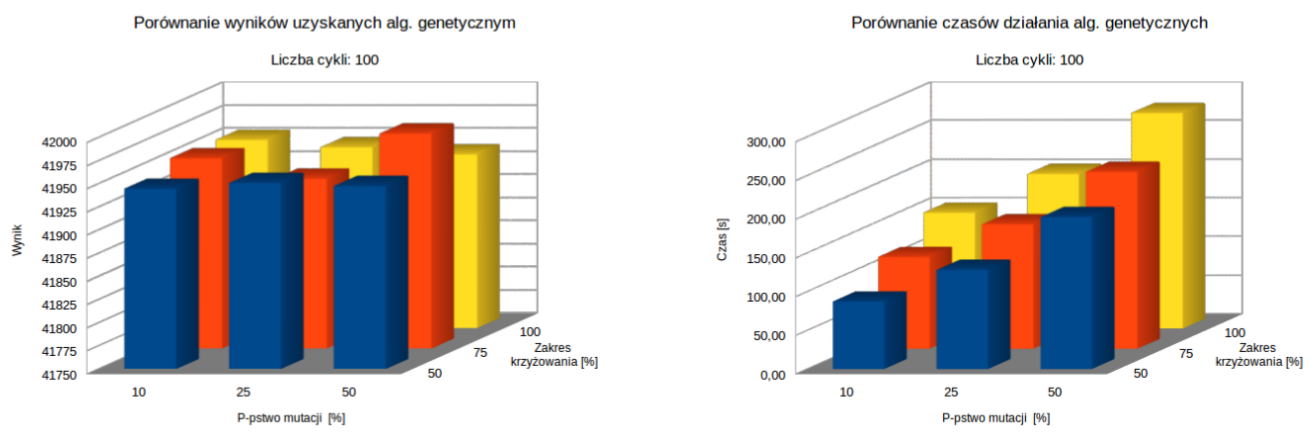
\includegraphics[width=0.8\paperwidth]{pics/gen100.png}

\end{frame}

%----------------------------------------------------------------------------------------

\subsection{Alg. zachłanny vs. genetyczny}

\begin{frame}
\frametitle{Alg. zachłanny vs. genetyczny}

\begin{itemize}

\item „Dobry” algorytm genetyczny (z wystarczająco wysokimi parametrami) zazwyczaj działa dłużej niż algorytm zachłanny
\item Wraz ze wzrostem parametru $p$ pogarsza się jakoś heurystyki w algorytmie zachłannym, stąd algorytm genetyczny zaczyna osiągać lepsze wyniki.

\end{itemize}

\end{frame}

%----------------------------------------------------------------------------------------

\section{Wdrożenie}


\begin{frame}
\frametitle{Wdrożenie aplikacji}

Aplikacja jest dostępna pod adresem:\\
\url{https://election-computing-system.herokuapp.com/}

\end{frame}

%----------------------------------------------------------------------------------------


\begin{frame}
\Huge{\centerline{Dziękujemy za uwagę}}
\end{frame}

%----------------------------------------------------------------------------------------

\end{document} 
